\subsection{Hybrid and Embedded Systems Theory} 

            %\subsubsection{Finite State Machines and Modal Models (Lee)}

            %Finite State Machines and Modal Models in Ptolemy II Finite-state machines (FSMs) and modal models provide a very expressive way to build up complex model behaviors. As a consequence of this expressiveness, it takes some practice to learn to use them well. Edward Lee has compiled a technical memorandum \cite{Lee:EECS-2009-151} that describes the usage and semantics of FSMs and modal models in Ptolemy II. 

            %FSMs are actors whose behavior is described using a finite set of states and transitions be-tween the states. The transitions between the states are enabled by guards, which are boolean-valued expressions that can reference inputs to the actor and parameters in scope. The transitions can produce outputs and can update the value of parameters in scope. Modal models extend FSMs by allowing states to have refinements, which are hierarchical Ptolemy II models. The re-finements may themselves be FSMs, modal models, or any composite actor containing a director compatible with the domain in which the modal model is being used. On the basis of several ex-amples, the memorandum describes the operational semantics, the practical usage, and the se-mantics of time in modal models. 

            %Each of the figures in the document corresponds to an executable Ptolemy II model. To exe-cute and experiment with these models the reader can simply click on the corresponding figures in the document. There is no need to pre-install Ptolemy II or any other software. 

            \subsubsection{Constructive Architectures for Digital Controllers of Continuous Time Systems (Kottenstette)}

Our overall research goal has been to create constructive networked control architectures for formation control of both quadrotor and fixed-wing aircraft which allows for collision avoidance while maintaining stability.  In order to obtain this goal we: 1) developed a constructive non-linear control framework which allows non-linear affine systems such as fixed-wing aircraft to be rendered strictly-output passive; 2) established a networked control architecture to interconnect multiple-agents in order to achieve a formation; and 3) modified a classic collision avoidance algorithm in order to achieve separation of aircraft.

\begin{enumerate}
\item Our first result applies to networked control of non-linear affine systems, including fixed wing aircraft, quadrotor aircraft, robotic, thermal, semiconductor manufacturing, alternative energy generation, and active suspension systems. These nonlinear affine systems can be expressed through what we term "m-Triangular Systems". The m-Triangular System renders possible a well-posed, distributed, continuous-time, control law which can be applied to nonlinear affine systems. This control law creates a strictly-output passive system which can then be integrated into a multirate discrete time networked control architecture. This robust architecture permits a discrete time strictly passive lag compensator to determine the desired output of the strictly-output passive system. Thus, we can integrate unmanned jet fighter aircraft into the NextGen system in which the lag compensator is located at the ground-control station. We can now safely control the inertial position of these aircraft despite communication time varying delays and data loss \cite{NK_1a,NK_1b,NK_1c}.
\item Our second result builds on our advanced digital networked control architecture in which passivity is preserved in spite time varying delays and data loss \cite{NK_2}.  The key to this architecture is our networking abstraction known as the power-junction and some minor analysis showing that it can be distributed over arbitrary overlay network topologies \cite{NK_3a,NK_3b}.  The overall architecture then allows for steady-state analysis in order to derive final formations of quadrotor aircraft.  These predicted results have been verified using our advanced Simulink based models of quadrotor aircraft in which time varying delays and data loss were simulated using TrueTime.  
\item Finally the classical collision avoidance algorithms \cite{NK_4a,NK_4b} had to be modified using a non-linear filtering architecture which is described precisely in \cite{NK_1a} and filtering architecture is inspired on the pioneering work of \cite{NK_5a,NK_5b,NK_5c}.
\end{enumerate}


            We have recently demonstrated how to interconnect either a linear or nonlinear interior-conic continuous time systems (in which passive systems are a special case) to an appropriately constrained conic digital controller in which continuous time stability ($L_m^2$-stability) can be guaranteed in spite of time-varying delay.  The key to achieving a stronger result and further weaken our initial passivity assumptions of the continuous time system is to explicitly consider the resulting conic-system properties resulting from the feedback loops created from our use of wave variables.  Initial results demonstrate improved rejection of high-frequency noise which can be effectively filtered with multi-rate passive samplers (PS:MTs) and passive hold devices (PH:M Ts) while achieving better performance over traditional sample-and-hold digital control systems.  As a result, we can now control the position of robotic arm manipulators using direct position feedback instead of indirect velocity feedback.  In addition we have shown that the inner-product-equivalent sampler and zero-order-hold (IPESH) not only preserves passivity properties of a given system but preserves the more general interior-conic system properties as well.  The implication is that like the bilinear-transform which preserves both passivity and stability properties when mapping a continuous linear time invariant (LTI) system to a discrete LTI system, the IPESH in general preserves stability for nonlinear interior conic systems such that if the IPESH is applied to a continuous interior conic system which is inside the sector $[a,b]$ then the resulting discrete-time system whose output is scaled by $\frac{1}{T_s}$) remains inside the sector $[a,b]$.  These results should extend to those related to control over power junction networks.

            We have demonstrated that a simplified linear power junction network can be used in distributed deployment of point-mass systems whose inertial position control system closely resembles that used to control position for our quadrotor aircraft.  Furthermore a resilient power junction network has also been demonstrated to allow a single plant to be reliably controlled by many redundant digital controllers in order to better withstand both denial-of-service (DOS) attacks and even safely handle certain compromises of the redundant controllers.  The linear power junction network appears to be a good candidate for networked control of quadrotor aircraft as well as fixed wing aircraft.

    In order to better study formation control of fixed wing aircraft for a potential aerial refueling scenario posed at our 2009 review we had to develop an inertial control system and model of a fixed wing aircraft.  Therefore we developed and verified an advanced Simulink-based fixed wing model of the Cessna A-37 whose velocity flight path and heading angles were maintained by a resilient backstepping control law.  The backstepping control law was derived using a simplifying small-angle assumption involving the angle of attack and bank angle while maintaining the side-slip angle near zero.  It achieves performance close to its adaptive counterparts while allowing for system model verification.  In addition we demonstrated that if we filter one of the feedback terms typically required to achieve asymptotic stability results for our backstepping controller then we could better withstand discrete time wind gusts.  In general we proved our backstepping control law can be applied not only to the control of fixed wing aircraft but other nonlinear systems which possess triangular structures and invertible controller affine terms.  Finally we demonstrated that a classical anti-windup compensator can be applied to the velocity control system when subject to control thrust saturation which can occur during aggressive maneuvers.  The small-angle assumption allowed us to significantly simplify our backstepping control law for our fixed wing aircraft, however, the quadrotor aircraft control system was still much less complicated.  Although both systems share the same kinematic equations of motion, the fixed wing aircraft dynamics depend heavily on the wind velocity vector.  As a result it is not clear how to exploit the passivity-like subsystems related to the kinematics in order to simplify the control design as was done for the quadrotor aircraft.  However, one technique to simplify controller design which looks promising is Interconnection Damping Assignment Passivity Based Control (IDA-PBC).

    IDA-PBC attempts to derive control laws which attempt to exploit the passivity-like properties of a system in order to derive a dissipative structure which achieves asymptotic stability.  Unlike backstepping control laws, IDA-PBC is not as aggressive in attempting to cancel non-linear terms in the system in order to make it appear as a cascade of integrators.  As a result the IDA-PBC control laws are typically less computationally intensive and possess more linear feedback terms similar to those seen with our quadrotor control system. We have studied, implemented and refined an IDA-PBC control algorithm initially presented by Johnsen \& Allgower related to the control of a four-tank process.  We have developed preliminary tools to automatically generate IDA-PBCs while providing improved integrator anti-windup compensators.  Furthermore we determined that the bilinear-transform works quite well in implementing low-sample-rate (possibly nonlinear) integrator terms in the IDA-PB controllers.  Furthermore IDA-PBC allows us to determine explicit gain and trajectory constraints to apply to our controller implementation in order to further improve system resilience.

\subsubsection{Robust Group Coordination}

For many sensing, surveillance, or tracking applications, it is often desirable to deploy a group of unmanned aerial vehicles (UAVs) for reconnaissance or scouting using coordination algorithms for decentralized control. Using large numbers of UAVs equipped with surveillance and sensing equipment is beneficial because redundancy reduces the likelihood of missing interesting events in the presence of obstructions caused by non-uniform terrain, man-made structures, or man-made interference. Therefore, we aim to develop methods that utilize decentralized control of UAVs to enhance security and redundancy for group coordination problems.

Performing coordinated tasks such as establishing a formation or output synchronization requires local interactions (e.g., via message passing) in a discrete-time framework for multi-agent systems. However network uncertainties such as delays and dropped packets introduce additional challenges to achieving the desired task. In particular, stability of the networked system can be jeopardized by these effects.  To circumvent the stability problems caused by the discrete-time implementation of multi-agent networks, a compositional approach has been created using passivity, which ensures $l_m^2$-stability of the global system whenever the individual components are passive.  Specifically, we have created and implemented an inherently distributed and passive communication architecture, which allows strictly-output passive, dynamical systems to be coupled through any discrete time overlay network in a stability-preserving manner, regardless of time-varying delays and data loss.

The specific problem we consider for our application of the passive communication architecture is the situation where $n$ agents distributed randomly in a two-dimensional environment attempt to create a formation surrounding a target position. Each agent has a neighborhood within which it is able to communicate, and no information is shared globally.

Fig. \ref{fig:consensus_3nodes} presents an example three node neighborhood communication scheme between nodes $i$, $j$, and $q$.  Each node sends position information encoded as a wave variable $u(k)$ to a delay state $d(k)$. The delay state passes the delayed information $v(k)$ as an input to the corresponding node.  The entire scenario is made of collections of these neighborhoods that have overlapping nodes.

               \begin{figure}[thpb]
 	         \centering
	         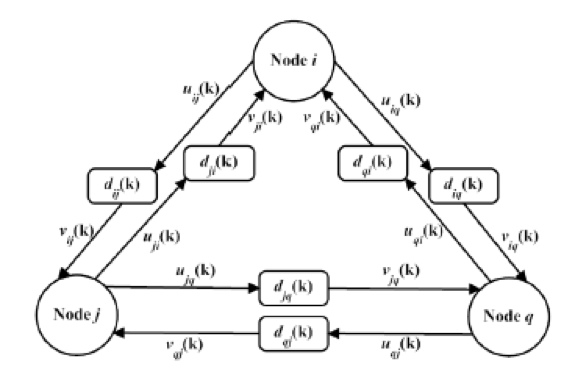
\includegraphics[width=0.9\textwidth]{img/consensus_3nodes}
	         \caption{An example 3-node communication network, illustrating the delay terminology.}
	         \label{fig:consensus_3nodes}
               \end{figure}



We have developed and tested (in simulation) the decentralized passivity and coordination algorithms for multiple UAV formation control.   We verified that the algorithms perform well in the presence of communication delays and dropouts, and have been shown to work well for systems even in the presence of large communication loss or delays.

               \begin{figure}[thpb]
 	         \centering
	         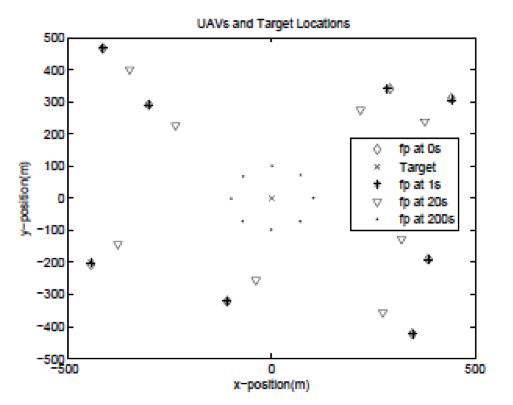
\includegraphics[width=0.9\textwidth]{img/consensus_sim}
	         \caption{Progression of UAVs to desired locations in presence of 10\% packet loss.}
	         \label{fig:consensus_sim}
               \end{figure}



One of our experimental scenarios involved a network of eight UAVs distributed in a regular lattice network structure.  Each UAV has four neighbors that it can communicate with using our passivity framework over the network, and we modeled a 10\% probability of packet loss. The scenario was modeled using Matlab and TrueTime for network communication simulation.  Fig. \ref{fig:consensus_sim} presents snapshots of the UAV positions at various times during the simulation.  It can be seen that the UAVs end up surrounding the target in the desired formation even with the network interference

            \subsubsection{Hierarchies of Robust Hybrid and Embedded Systems (Tomlin, Krogh, Sastry)} 
               
               \textit{Reachability Analysis.}  In safety-critical
               applications, the task of controller design and
               synthesis is often subject to hard constraints such as
               safe operation envelopes, target attainability
               requirements, and limits on the admissible control
               inputs.  Furthermore, due to various uncertainties in
               the modeling phase and operation phase, the controller
               design must be robust to factors such as modeling
               error, environment disturbances, and adversarial
               actions.

               Over the course of this MURI, we have developed several
               methods for addressing these problems in the context of
               a hybrid system abstraction, which is a powerful
               modeling framework encapsulating both continuous and
               discrete dynamics.  Our approach is based upon a
               dynamic game formulation of reachability analysis in
               which the safety and target attainability objectives
               are encoded as reachability objectives, and the
               disturbance is modelled as an adversarial agent.  In
               the following, we will briefly outline some of these
               methods, along with relevant application scenarios.

               \emph{a) Provably Safe Maneuver Sequence Design}

               In the case where the sequence of transitions in a
               hybrid system is known ahead of time, we have developed
               a systematic method for designing the discrete
               transition conditions, as well as the continuous
               control laws so as to satisfy a given safety
               specification
               \cite{c:ding-CDC-2008,j:ding-aiaa-gnd-2011}.  This
               method is applied to the problem of flight maneuver
               design for automated aerial refueling (AAR) .  This
               scenario arises when unmanned aerial vehicles (UAVs)
               undertake long range missions need to be refueled
               mid-flight by a human-operated tanker aircraft.  The
               refueling procedure is illustrated in
               Figure~\ref{fig:AAR_Diagram}.

               \begin{figure}[thpb]
 	         \centering
	         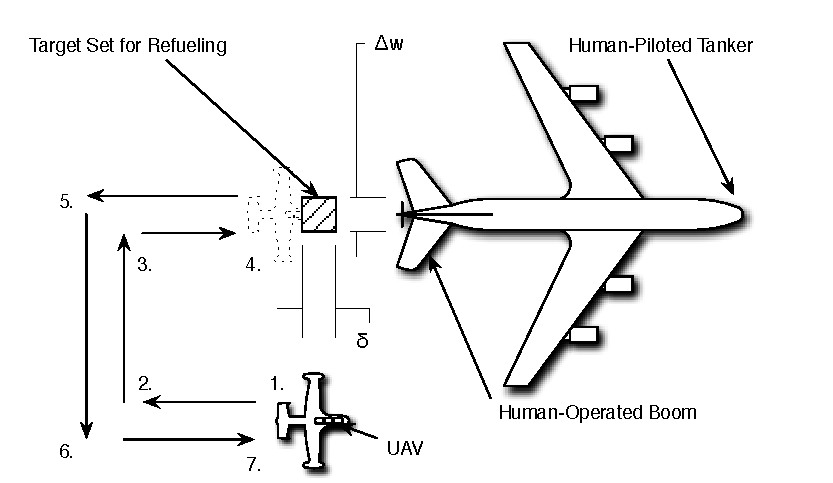
\includegraphics[width=0.7\textwidth]{img/overhead-crop}
	         \caption{Automted aerial refueling sequence.}
	         \label{fig:AAR_Diagram}
               \end{figure}

               Under a hybrid system abstraction, the discrete modes
               are the flight maneuvers performed in transitioning
               between the waypoints labeled in
               Figure~\ref{fig:AAR_Diagram}, while the continuous
               states are the relative coordinates of the tanker
               aircraft in the UAV reference frame, represented by a
               vector $x = (x_1, x_2, x_3)$ (the longitudinal,
               lateral, and heading coordinates, respectively). The
               relative motion between the tanker aircraft and UAV is
               then described by a kinematics model of the form
               $\dot{x}=f(x,u,d)$, where $u$ is the control input (in
               this case the translational and angular velocities of
               the UAV), and $d$ is the disturbance entering into the
               system (in this case the fluctuation in tanker velocity
               due to wind effects).

               The maneuver sequence design problem involves choosing
               the switching conditions between the flight maneuvers,
               as well as the continuous control laws for the input
               $u$, so as to ensure that a collision between UAV and
               tanker is prevented regardless of possible environment
               disturbances $d$ and command latencies.  Under our
               proposed approach, a reachability calculation is
               carried out for each flight maneuver in the refueling
               sequence to determine 1) the capture set, which is the
               set of aircraft states from which a target waypoint can
               be attained within a finite time horizon, and 2) the
               collision set, which is the set of aircraft states from
               which the trajectory of a flight maneuver passes
               through a collision zone centered on the tanker
               aircraft.  An example of these sets computed for the
               Precontact maneuver (transition between waypoints 2 and
               3) is shown in Figure~\ref{fig:reachset_Precontact}.

               \begin{figure}[thpb]
 	         \centering
	         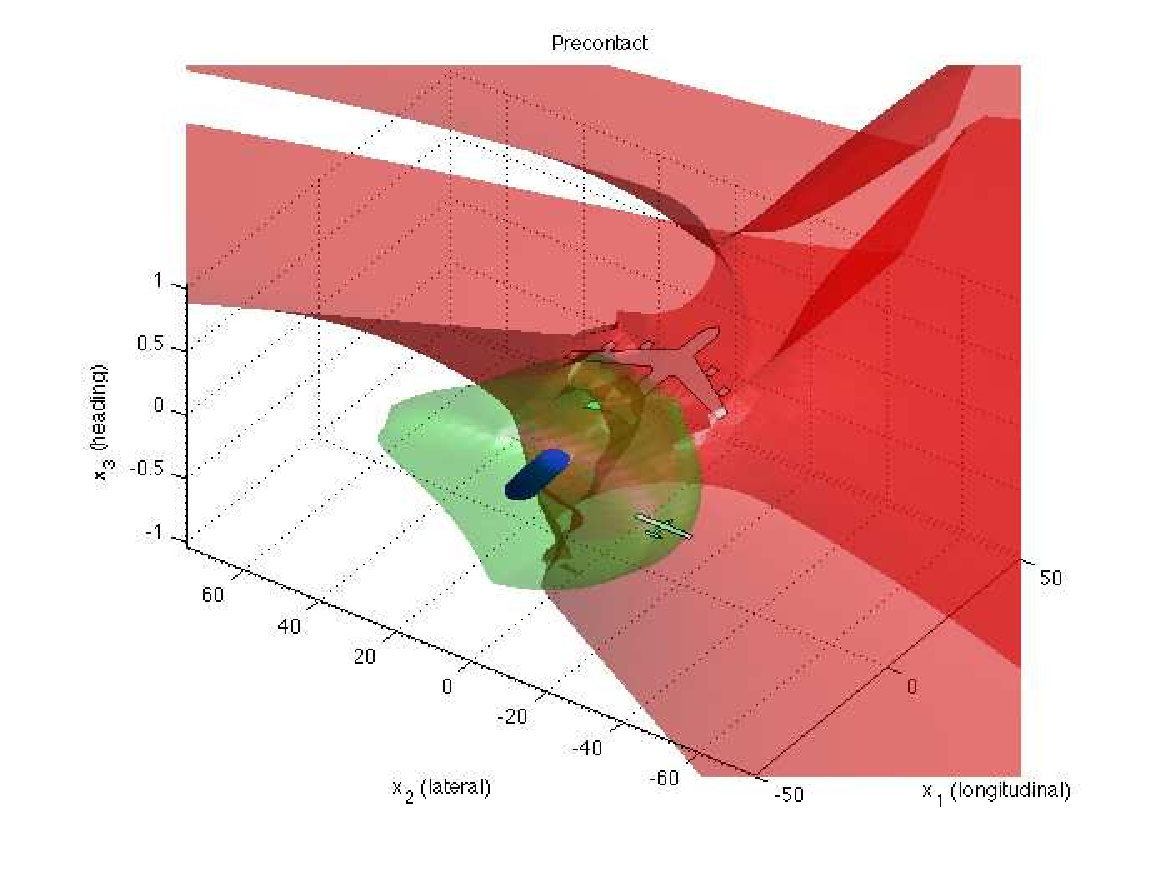
\includegraphics[width=0.7\textwidth]{img/reachset-precontact}
	         \caption{Capture set (light, green) and collision set (dark, red) computed for Precontact maneuver in aerial refueling sequence.}
	         \label{fig:reachset_Precontact}
               \end{figure}

               At design time, the capture sets and collision sets
               computed for the various maneuvers in the AAR sequence
               can be used to guide the choice of maneuver control
               laws and switching conditions to ensure that each
               maneuver terminates in an aircraft state that satisfies
               the target-attainability and safety objectives of the
               next maneuver (thus allowing the next maneuver to be
               feasibly initiated). Furthermore, through appropriate
               modifications of the reachability analysis, the effects
               of bounded disturbances and communication latency can
               also be taken into account. However, in such cases, the
               resulting design of maneuver control laws and switching
               conditions is in general more conservative than the
               case in which the robustness factors are not
               considered.  The performance of the control laws and
               switching conditions for the full AAR sequence has been
               validated in simulation with realistic model
               parameters, as detailed in \cite{j:ding-aiaa-gnd-2011}.


               \emph{b) Automatic Controller Synthesis for Switched Nonlinear Systems}

               While in certain applications a mode sequence is
               specified a priori according to designer insights,
               there are many cases in which one is simply given a set
               of controlled modes of operation and the task is to
               construct a mode selection policy, possibly as function
               of the state measurements, so as to ensure that desired
               control objectives are satisfied.  In particular,
               consider a switched nonlinear system of the following
               form:
               \begin{equation}
                 \label{eq:switched}
                 \dot{x}(t) = f_{q(t)}(x(t), u(t), d(t))
               \end{equation}
               where $\left\{f_q, q \in Q\right\}$ is a family of
               vector fields parametrized by a finite index set $Q$
               (for example a finite set of flight maneuvers); $u$ is
               a continuous control input; and $d$ is a disturbance
               input.

               We are interested in synthesizing controllers, which
               involves both a choice of the discrete mode $q$ and the
               continuous input $u$, so as to drive the continuous
               state $x$ into a set of goal configurations $R$, while
               avoiding an unsafe set $A$, subject to system dynamics
               (\ref{eq:switched}) and unknown but bounded,
               time-varying disturbances.  We call this a
               \textit{reach-avoid} problem.  For practical
               considerations, the controller is alllowed to modify
               input selections only at regularly spaced sampling
               instants, $t=0,T,...,NT$, at which measurements of the
               system state are received.

               In \cite{c:ding-CDC-2010} and \cite{c:ding-ICRA-2011},
               a solution to this controller synthesis problem is
               proposed, based upon iterative reachability
               calculations over sampling intervals.  In particular,
               we compute over successive iterations $k = 0,1,...,N$,
               the set of initial conditions $S_k$ for which there
               exists an admissible feedback policy satisfying the
               reach-avoid objectives over $[0,kT]$, subject to the
               worst-case disturbance, using a differential game
               formulation of reachability analysis.  The resulting
               set $S_N$ then provides us with the $N$-step feasible
               set for the reach-avoid problem.  Furthermore, as
               discussed in \cite{c:ding-CDC-2010}, we can derive from
               the representation of the sets $S_k$ a set-valued
               control law which satisfies the desired control
               objectives over $[0,kT]$.  By storing the reachable
               sets as lookup tables, one can then compute the
               appropriate control inputs in an online setting by
               checking set inclusions.  It has also been shown that a
               variant of this reachability calculation can be used to
               address the invariance problem, in which the objective
               is to remain within a desired set indefinitely
               \cite{c:ding-ICRA-2011}.

               We have applied this controller synthesis approach in
               an experimental setting to a target tracking problem,
               in which the objective is to control a quadrotor
               helicopter to first hover over a stationary ground
               vehicle and then track the vehicle as it starts moving,
               while satisfying certain velocity constraints.  In this
               case, the modes of the system are used to represent
               discrete choices of roll and pitch angles, which
               affects the quadrotor acceleration in the $x$ and $y$
               directions, while disturbances appear in the form of
               model uncertainties, as well as the movement of the
               ground vehicle, which is not planned ahead of time.

               Using the procedure described previously, we computed
               the set of initial conditions in the relative
               position-velocity space reachable to the hover region
               over 2.5 seconds, with the results shown in Figure
               \ref{fig:target_tracking}(a).  The control policy
               derived from this reachability computation was then
               implemented onboard the Stanford Testbed of Autonomous
               Rotorcraft for Multi-Agent Control (STARMAC).  The
               trajectories from an experimental run are shown in
               Figure \ref{fig:target_tracking}(b).  It can be seen
               that the quadrotor indeed enters the hover region
               within the time horizon of interest, and then remains
               within this region for the rest of the experiment,
               despite movements of the ground vehicle.
               \begin{figure}[thpb]
 	         \centering
	         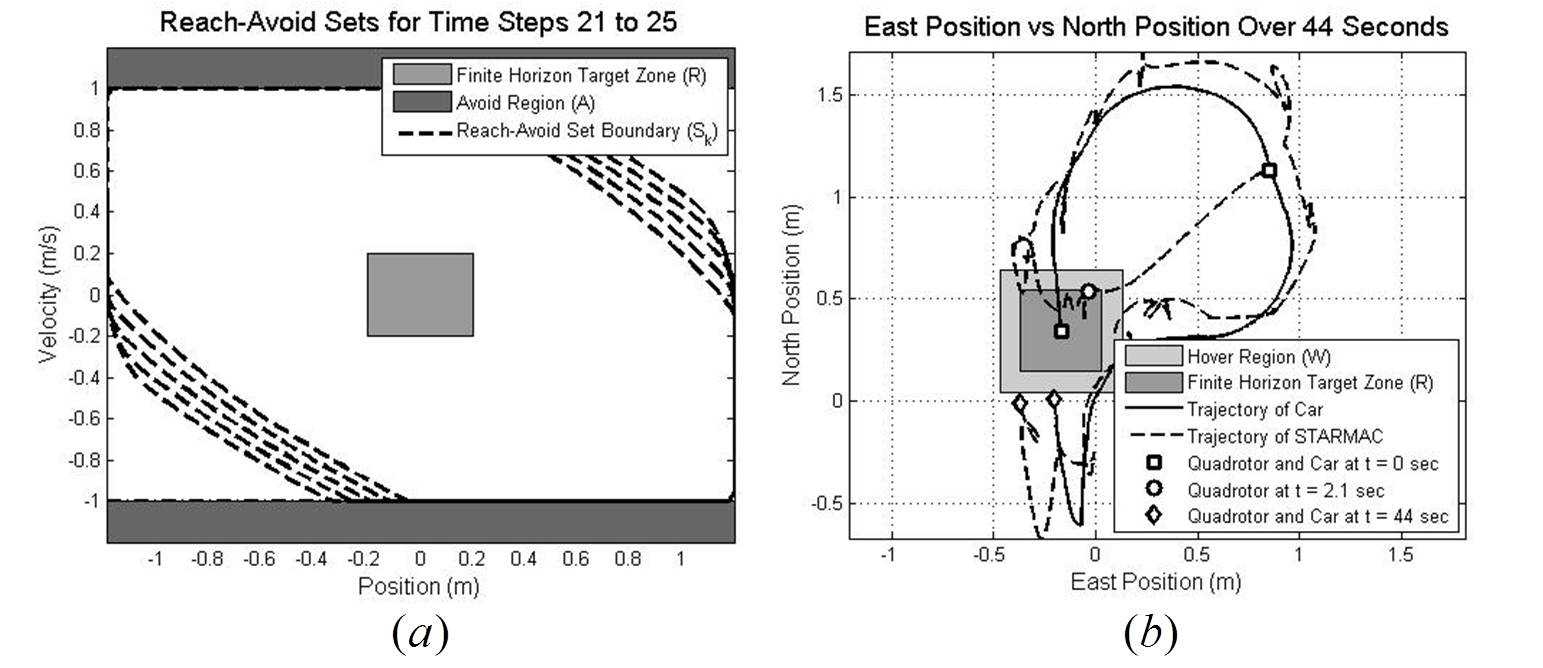
\includegraphics[width=0.9\textwidth]{img/target-tracking-plots}
	         \caption{Results for target tracking application: (a) reach-avoid sets in position-velocity space over 2.5 seconds ($T = 0.1$ s); (b) experimental trajectories of quadrotor and ground vehicle.}
	         \label{fig:target_tracking}
               \end{figure}



\subsubsection{Optimal Control of Switched Hybrid Dynamical Systems (Sastry, Tomlin)}

A natural extension of classical dynamical systems, where the state of the system is governed by a single differential equation, are switched dynamical systems, where the state of a system is governed by a finite number of differential equations, each of which can be arbitrarily chosen at an instant of time. The control parameter for such systems has a discrete component, the sequence of modes, and two continuous components, the duration of each mode and the continuous input. Switched systems arise in numerous modeling applications \cite{brockett1995stabilization, rantzer_switch}. 

Stemming from Branicky et al.'s seminal work that established a necessary condition for the optimal trajectory of switched systems in terms of quasi-variational inequalities \cite{branicky1998ufh}, there has been growing interest in the optimal control of such systems. However, Branicky provided only limited means for the computation of the required control. Others have employed variants of dynamic programming to develop algorithms to address the special case of piecewise-linear or affine systems \cite{bemporad2000piecewise,borrelli_hybrid,giua2001optimal}. Since after each iteration of these algorithms the number of possible switches grows exponentially, the representation of the optimal value function becomes increasingly complex. These approaches focus on addressing this particular shortcoming by considering a variety of possible relaxations of the optimal value function. 

Several address just the continuous component of the optimal control of an unconstrained nonlinear switched system while keeping the sequence of modes fixed. Given a fixed mode schedule, Xu et al. develop a bi-level hierarchical optimization algorithm:  at the higher level, a conventional optimal control algorithm finds the optimal continuous input assuming fixed mode duration and at the lower level, a conventional optimal control algorithm finds the optimal mode duration while keeping the continuous input fixed \cite{xu2003}. Axelsson et al. consider the special case of unconstrained nonlinear autonomous switched systems (i.e. systems wherein the control input is absent) and develop a similar bi-level hierarchical algorithm: at the higher level, the algorithm updates the mode sequence by employing a single mode insertion technique, and at the lower level, the algorithm assumes a fixed mode sequence and minimizes the cost functional over the switching times \cite{axelsson2008,egerstedt2006}. 

We generalized Axelsson's approach by constructing an optimal control algorithm for constrained nonlinear switched dynamical systems \cite{gonzalez2010descent, gonzalez2010cdc}. In our first paper we developed a bi-level hierarchical algorithm that divided the problem into two nonlinear constrained optimization problems. At the lower level, our algorithm assumed a fixed modal sequence and determined the optimal mode duration and optimal continuous input. At the higher level, our algorithm employed a single mode insertion technique to construct a new lower cost sequence. The result of our approach was an algorithm that provided a sufficient condition to guarantee the local optimality of the mode duration and continuous input while decreasing the overall cost via mode insertion. Though this was a powerful outcome given the generality of the problem under consideration, it suffered from three shortcomings which made its immediate application difficult. First, if our algorithm was initialized at an infeasible point it was unable to find a feasible lower cost trajectory. Unfortunately, initializing an optimization algorithm with a feasible point is nontrivial. Second, our algorithm did not incorporate multiple objectives into its cost function, which is useful for path planning type tasks. Finally, our algorithm did not penalize the number of hybrid jumps. In our second paper we design a new algorithm to address these three deficiencies and detail the utility of this modified approach on two examples.


We are interested in the optimal control of dynamical systems whose trajectory is governed by a differential equation of the form:
\begin{equation}
  \dot{x}(t) = f\big( x(t), u(t), d(t) \big), \quad \forall t\geq0,\quad x(0) = x_0,
\end{equation}
where $u: [0,\infty) \to \mathbb{R}^m$ is continuous input and $d: [0,\infty) \to \{ 1, 2, \ldots, Q \}$ is the discrete input. Instead of directly optimizing over the discrete input $d$, we optimize over the sequence $\sigma: \mathbb{N} \to \{ 1, 2, \ldots, Q \}$ and $s: \mathbb{N} \to [0,\infty)$, where it must be noted that given a pair $(\sigma,s)$ one can construct a discrete input recursively by, given $k \in \mathbb{N}$, applying the input $\sigma(k)$ for $s(k)$, and then repeat replacing $k$ with $k+1$. Also, since we want to account for several objectives as mentioned above, we introduce a extra variable $w: \{ 1, 2, \ldots, W \} \to \mathbb{N}$ which indexes the objectives.

Our algorithm finds a numerical solution of the following problem:
\begin{flalign}
  & {(OCP)} & 
  & \min_{ \sigma, s, u, w }\ \int_0^T L \big( x(t), u(t), t \big) dt + \sum_{k=1}^W \phi_k\big( x( \tau_{w(k)} ) \big) + C \#\sigma, & 
  & 
\end{flalign}
subject to:
\begin{align}
  & \tau_k = \sum_{i=1}^k s(i),\\
  & \dot{x}(t) = f\big( x(t), u(t), d(t) \big), \quad t \in [0,T], \quad x(0) = x_0,\\
  & \text{$d$ is constructed from the pair $(\sigma,s)$,}\\
  & h_j\big( x(t) \big) \leq 0, \quad \forall t \in [0,T], \quad j \in \{ 1, 2, \ldots, J \}.
\end{align}
The problem $(OCP)$ has both continuous as well as discrete variables, thus it is usually solved numerically using Integer Programming algorithms, which suffer the curse of dimensionality, i.e. as the size of the discrete variable increases linearly the number of function evaluations increases exponentially. Our algorithm offers numerical solutions which are not strict minimizers (i.e. our algorithm might stop at points that are not necessarily global minimizers) but it does not suffer the curse of dimensionality.

The algorithm solves a two-level optimization problem. In the first level it fixes $\sigma$ and $w$ and it minimizes $s$ and $u$ using known optimal control techniques as the ones in \cite{polak1997}. The second level performs a first-order variation of the cost function after the instantaneous insertion of an extra mode at a particular time: if the variation results in a decrease of the cost, then create a new sequence $\sigma$ including that insertion and repeat the process. This procedure converges to a class of points where the first-order variation produces no change in the cost, and hence no single mode insertion can further decrease the cost \cite{gonzalez2010descent, gonzalez2010cdc}.

As an example, we consider the optimal control of a quadrotor helicopter in 2D using a model described in \cite{gillula2011applications}. The evolution of the quadrotor can be defined with respect to a fixed 2D reference frame using six dimensions where the first three dimensions represent the position along a horizontal axis, the position along the vertical axis and the roll angle of the helicopter, respectively, and the last three dimensions represent the time derivative of the first three dimensions. We model the dynamics as a three mode switched system (the first mode describes the dynamics of going up, the second mode describes the dynamics of moving to the right, and the third mode describes the dynamics of moving to the left) with a single input as described in Table \ref{tab:ocp_dynamics} where $L = 0.305$ meters, $M = 1.3$ kilograms, $I = 0.0605$ kilogram meters squared and $g = 9.8$ meters per second squared. The cost and input constraints are as described in Table \ref{tab:ocp_cost} where the waypoints, $\hat{w}(i)$, are:
\begin{equation}
	\hat{w}(1) = 
  \begin{bmatrix} 
    2 \\ 5 \\ \pi 
  \end{bmatrix} 
  \ \text{and}\  
  \hat{w}(2) = 
  \begin{bmatrix} 
    4 \\ 1 \\ 0 
  \end{bmatrix},	
\end{equation}
and the time-varying desired trajectory is defined as:
\begin{equation}
	r(t) = 
	\begin{cases}
		(t,1), & \mbox{ if } t < 2 \\ 
		(2+\cos\left(t - 2 - \frac{\pi}{2}\right), 3+2\sin\left(t - 2 - \frac{\pi}{2}\right), & \mbox{ if } t < 2 + 2\pi \\
		(t-2+2\pi,1), & \mbox{ if } t < 4 + 2\pi \\
		(4,1), & \mbox{ else }
	\end{cases}
\end{equation}
The state is constrained to remain above the ground and outside of a box of height and width both equal to $1$ centered at $(1,1)$. The result of iterations $1$, $7$, and $10$ of the algorithm are shown in Figure \ref{fig:starmacexample}.


\begin{table}[t]
  \begin{center}
    \begin{tabular}{cc}
      Mode 1: & 
      $\ddot{x}(t) = \begin{bmatrix} \frac{\sin x_3(t)}{M}\left( u(t) + Mg \right) \\	\frac{\cos x_3(t)}{M}\left( u(t) + Mg \right) - g \\ 0 \\ \end{bmatrix}$ \\
      Mode 2: & 
      $\ddot{x}(t) = \begin{bmatrix} g\sin x_3(t) \\ g\cos x_3(t) - g \\ \frac{-L u(t)}{I} \\ \end{bmatrix}$ \\
      Mode 3: &
      $\ddot{x}(t) = \begin{bmatrix} g\sin x_3(t) \\	g\cos x_3(t) - g \\ \frac{L u(t)}{I} \\ \end{bmatrix}$ \\
    \end{tabular}
  \end{center}
  \caption{The dynamics of each of the modes of the quadrotor for our example.}
  \label{tab:ocp_dynamics} 
\end{table}

\begin{table}[t]
  \begin{center}
    \begin{align*}
      L(x(t),u(t),t) &= 10 \sum_{j=1}^2 \big(x_j(t) - r_j(t) \big)^2 \\
      \phi_k \big( x( \tau ) \big) &= 100 \sum_{j=i}^2 \big( x_j(\tau) - \hat{w}_j(i) \big)^2 + 1000 \left( \sin^2 \left( \frac{x_3(\tau) - \hat{w}_3(i)}{2} \right) \right) \\
      C &= 1
    \end{align*}
  \end{center}
  \caption{The components of the cost function, the input constraints, and the parameters of the optimality function for our example.}
  \label{tab:ocp_cost}
\end{table}


\begin{figure}[!t]
  \begin{minipage}{\columnwidth}
    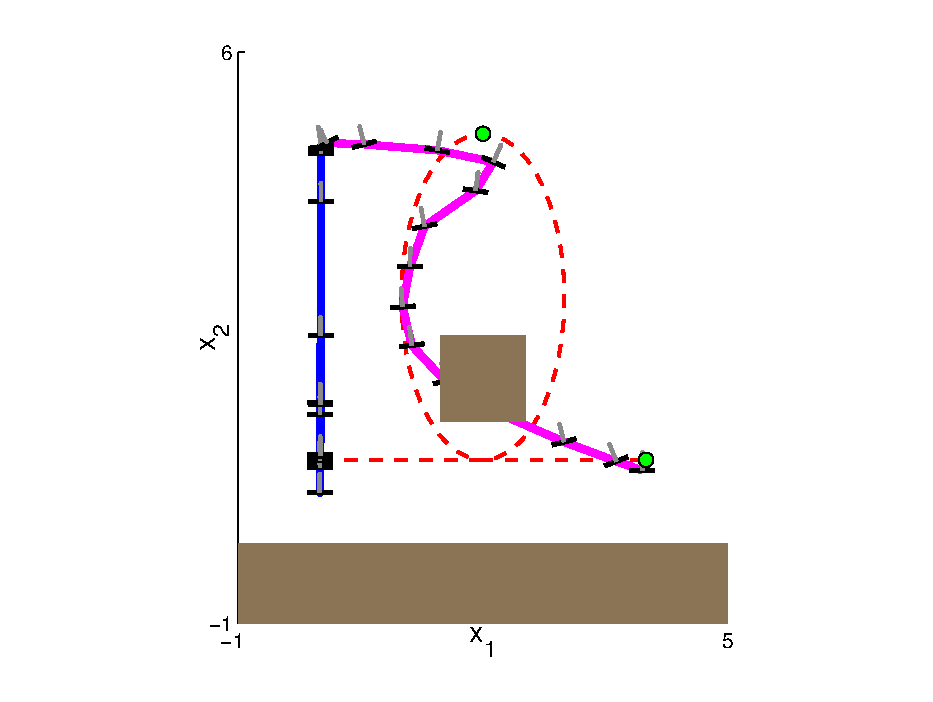
\includegraphics[clip, trim = 3.25cm .75cm 3.25cm .75cm, width = .32\columnwidth, keepaspectratio = true]{img/starmac_wp2_iter1}
    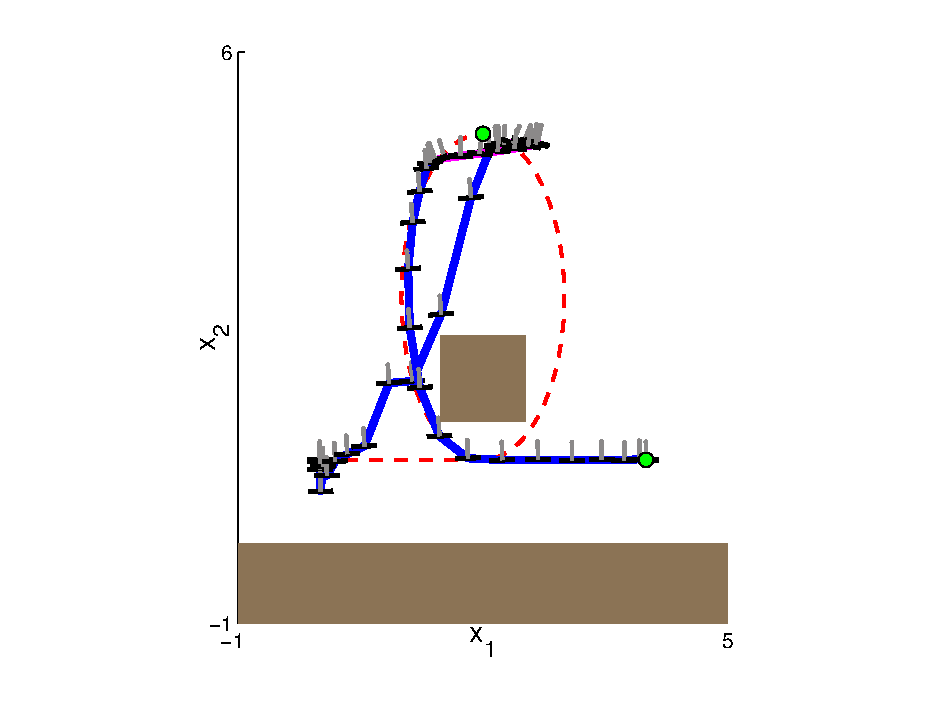
\includegraphics[clip, trim = 3.25cm .75cm 3.25cm .75cm, width = .32\columnwidth, keepaspectratio = true]{img/starmac_wp2_iter7}
    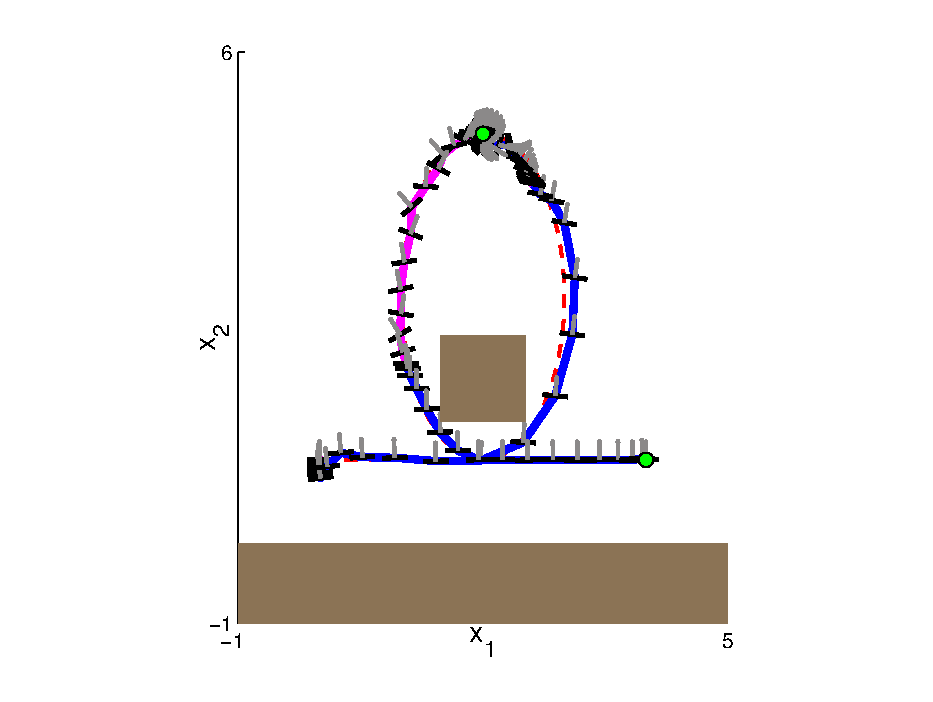
\includegraphics[clip, trim = 3.25cm .75cm 3.25cm .75cm, width = .32\columnwidth, keepaspectratio = true]{img/starmac_wp2_iter10}
  \end{minipage}
  \caption{Optimal trajectories (the quadrotor is drawn in black and the normal direction to the frame is drawn in gray) on the top row and bottom left in an environment with constraints (drawn in brown) and objectives (drawn in green). The first image shows iteration 1, the second iteration 7, and the third is iteration 10.}
  \label{fig:starmacexample}
\end{figure}


%%%%%%%%%%%%%%%%%
%%%%%%%%%%%%%%%%%
\subsubsection{Embedded Systems Modeling and Deep Compositionality (Krogh, Tomlin, Sastry)}
                 
                 \emph{Verification of Stochastic Hybrid Systems}
                 %    \newline \small{ Graduate Student: Maryam Kamgarpour}

                 \begin{figure}[!t]
                   \begin{center}
                     \begin{subfigmatrix}{2}% number of columns
                       \subfigure[Reach-Avoid problem]{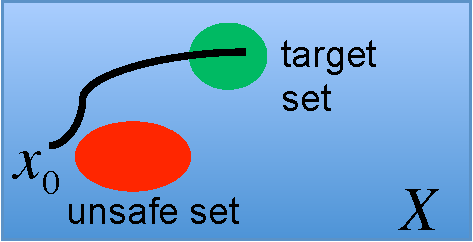
\includegraphics{img/reachavoidsets.pdf}}                
                       \subfigure[Probabilistic backward reach-avoid set]{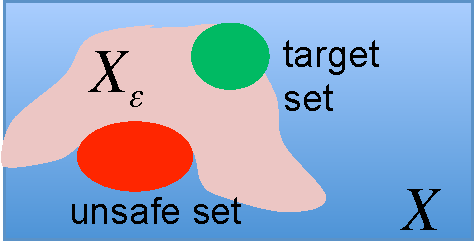
\includegraphics{img/reachavoidoptimal.pdf}}
                     \end{subfigmatrix}   
                     \caption{Reach-avoid problem for stochastic hybrid systems}
                     \label{fig:reach_avoid_problem}
                   \end{center}
                 \end{figure}

         

                 We consider a general hybrid modeling framework in
                 which we account for stochastic disturbances in
                 evolution of the continuous and discrete states. In
                 addition, we account for deterministic disturbances
                 in the model. The motivation is that while some
                 classes of uncertainty, such as those by nature, are
                 best modeled stochastically, some other classes of
                 uncertainty, such as those due to presence of agents
                 with competing objectives, are best modeled in a
                 deterministic worst-case approach. For example, in a
                 collision avoidance scenario between two aircraft, on
                 the one hand, wind affects the dynamics of aircraft
                 and uncertainties in wind forecast and measurement
                 may be best accounted for through a stochastic
                 framework. On the other hand, in the absence of
                 communication between the aircraft, from the
                 perspective of each aircraft, the trajectory must be
                 safe in the worst-case performance of the other
                 aircraft. Hence, a robust approach should be
                 considered.

                 The reach-avoid objective in the setting of the
                 stochastic hybrid system with two players becomes a
                 stochastic game in which the objective of player 1
                 (the control) is to steer the hybrid system state
                 into a desired target set, while avoiding a set of
                 unsafe states, as shown in Figure
                 \ref{fig:reach_avoid_problem}(a).  On the other hand,
                 the objective of player 2 (the adversary) is to
                 either steer the state into the unsafe set or prevent
                 it from reaching the target set.

                 Mathematically, the problem is stated as follows: Let
                 $X$ denote the hybrid state space. Suppose that Borel
                 sets $G, S \in \mathcal{B}(X)$ are given as the
                 desired target set and safe set, respectively, with
                 $G \subseteq S$.  Then the probability that the state
                 trajectory $(x_0, x_1, \dots, x_N)$ reaches $G$ while
                 staying inside $S$ under fixed choices of player 1
                 policy $\mu \in \mathcal{M}_a$ and player 2 strategy
                 $\gamma \in \Gamma_d$ is \cite{kamgar2011cdc}:

                 \begin{align*}
                   \label{eq:reachavoid_prob_expectation}
                   r_{x_0}^{\mu, \gamma}&(G,S) = E^{\mu,\gamma}_{x_0} \left[ \mathbf{1}_G(x_0) + \sum^{N}_{j=1}\left(\prod^{j-1}_{i=0}\mathbf{1}_{S\setminus G}(x_i)\right)\mathbf{1}_G(x_j)\right],
                 \end{align*}
                 where $E^{\mu,\gamma}_{x_0}$ denotes the expectation
                 with respect to the probability measure
                 $P_{x_0}^{\mu, \gamma}$ induced by the initial
                 condition, $x_0 \in X$, and the players'
                 strategies. The admissible control spaces consist of
                 the set of Markov policies and strategies, denoted by
                 $\mathcal{M}_a$, $\Gamma_d$, for the control and
                 adversary, respectively.

                 Define the worst-case reach-avoid probability under a
                 choice of Markov policy $\mu$ as $r_{x_0}^\mu(G,S) =
                 \inf_{\gamma \in \Gamma_d} r_{x_0}^{\mu,
                   \gamma}(G,S).$ Our objective is to maximize this
                 worst-case probability over the set of Markov
                 policies. Thus, we need to compute the maxmin value
                 function $r_{x_0}^*(G,S) := \sup_{\mu \in
                   \mathcal{M}_a} r_{x_0}^\mu(G,S)$, and find a maxmin
                 policy $\mu^* \in \mathcal{M}_a$, such that
                 $r_{x_0}^*(G,S) = r_{x_0}^{\mu^*}(G,S)$, $\forall x_0
                 \in X$.

                 We have developed a dynamic programming algorithm for
                 maximizing the reach-avoid probability and for
                 synthesizing a control law that achieves this
                 probability. In addition, from this algorithm we can
                 find the set of initial conditions $X_\epsilon$ for
                 which the reach-avoid probability is above
                 $(1-\epsilon)$, $\forall \epsilon \in [0,1]$, under
                 the worst-case adversary behavior, as shown in Figure
                 \ref{fig:reach_avoid_problem}(b).

                 The algorithm has been applied to several robust
                 motion planning problems including a quadrotor
                 helicopter tracking a ground vehicle and aircraft
                 conflict detection and resolution scenarios
                 \cite{kamgar2011cdc}.

                 \emph{Aircraft Conflict Detection}

                 The scenario involves two aircraft with possibly
                 intersecting nominal trajectories. From the
                 perspective of the first aircraft, the task is to
                 detect the possibility of conflict given current
                 position of another aircraft, and design a collision
                 avoidance trajectory in case potential conflict is
                 detected. Motivated by wind influence on aircraft
                 trajectories and on accuracy of conflict detection,
                 we consider wind with a deterministic component,
                 known through forecast or measurements, and a
                 stochastic component to capture its
                 uncertainties. Based on geostatistics analysis of
                 wind data, the stochastic wind component is modeled
                 as a time dependent random field over the $2D$
                 airspace.

                 A conflict is defined if aircraft get closer than a
                 critical distance of $R_c$. Hence, the safe set in
                 $2D$ can be defined in relative coordinates as: $S =
                 \{ (x^1,x^2) \in \mathbb{R}^2 \; s. t. \; \|
                 (x^1,x^2) \|_2 \geq R_c \}$.For conflict detection,
                 we assume that the current position of each aircraft
                 is available, for example through Automatic Dependent
                 Surveillance-Broadcast (ADS-B) network. For the
                 conflict resolution, we assume that the control of
                 the two aircraft are decentralized. Furthermore, in
                 the absence of further information on the decision
                 algorithms, each aircraft assumes that the other
                 aircraft could potentially make choices that endanger
                 safety.


                 The aircraft kinematics is modeled as a unicycle. The
                 input of each aircraft is its heading angle
                 rate. Motivated by discrete maneuvers used in air
                 traffic, we assume at any given time, each aircraft
                 can choose to be in one of three flight maneuvers:
                 straight, right turn, or left turn.

                 \begin{figure}[!t]
                   \begin{center}
                     \begin{subfigmatrix}{2}
                       \subfigure[Maxmin probability of safety]{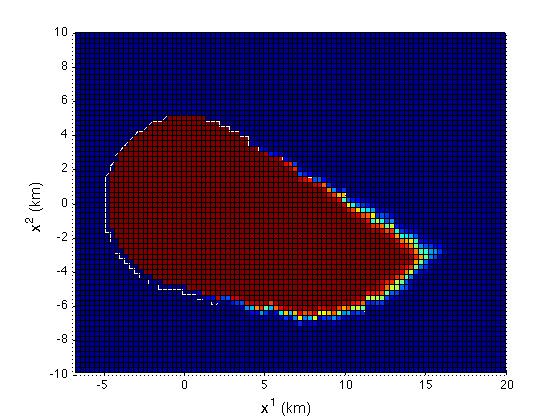
\includegraphics{img/pminmax_3pi4}}                
                       \subfigure[Deterministic reachable set]{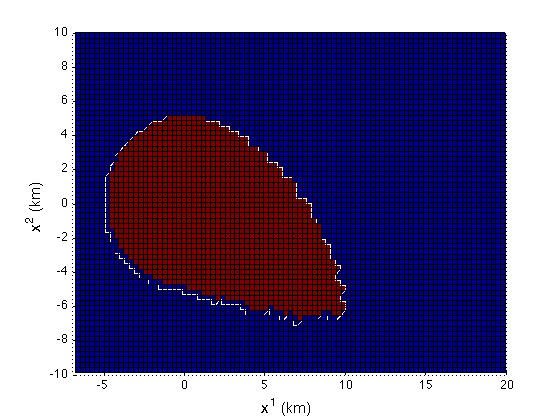
\includegraphics{img/deterministic_3pi4}}
                     \end{subfigmatrix}
                     \caption{Collision detection in probabilistic and deterministic settings}
                     \label{fig:prob_collision1}
                   \end{center}
                 \end{figure}

                 The maxmin probability of safety over a horizon of
                 $2.5$ minutes and with aircraft speed of $5$ km per
                 minute, is computed based on our proposed dynamic
                 programming algorithm. Figure
                 \ref{fig:prob_collision1}(a) illustrates this
                 probability for the set of initial conditions with
                 relative heading of $\frac{3\pi}{4}$ radians. The
                 interpretation of this probability map is as
                 follows. Consider an initial condition of $(10.55
                 \text{ km}, -6.85 \text{ km},\frac{3\pi}{4} \text{
                   rad})$. From the value function we obtain the
                 maxmin probability of safety to be $99 \%$.  This
                 means that if aircraft 1 selects flight maneuvers
                 according to the maxmin policy $\mu^*$ and aircraft 2
                 selects any maneuvers within the set of Markov
                 strategies, the probability of collision would remain
                 at most $1 \%$. For comparison, the result of
                 deterministic computation, in which wind influence is
                 ignored, is shown in Figure
                 \ref{fig:prob_collision1}(b). In this case, any
                 initial condition is characterized as being safe or
                 not.

                 \emph{Uncertain Safe and Target Sets}

                 \begin{figure}[!t]
                   \begin{center}
                     \begin{subfigmatrix}{2}
                       \subfigure[VIL measurements from forecast]{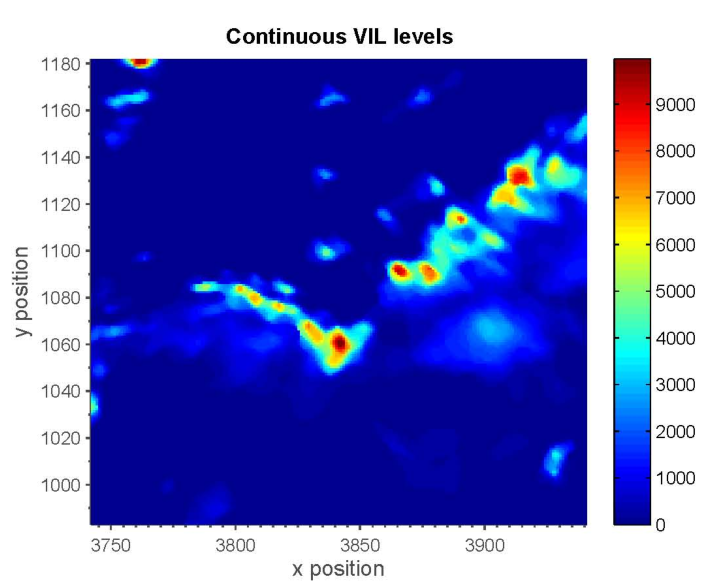
\includegraphics{img/VILcontinuous}}                
                       \subfigure[No-fly zones based on forecast]{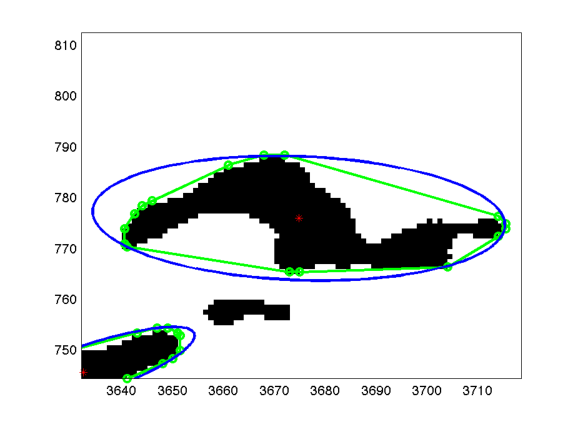
\includegraphics{img/VILenclosed}}
                     \end{subfigmatrix}
                     \caption{Forecast data for Vertically Integrated Liquid level}
                     \label{fig:vil}
                   \end{center}
                 \end{figure}

                 It has been shown that high values of Vertically
                 Integrated Liquid (VIL) level indicate storm
                 precipitation and regions with high VIL levels should
                 be avoided by pilots. We have used MIT Lincoln lab
                 forecast of VIL data over a gridded United States
                 airspace to characterize obstacles in aircraft
                 flight. Figure \ref{fig:vil}(a) shows the forecast
                 data for 01/07/2009 near gulf coast of Florida, while
                 Figure \ref{fig:vil}(b) shows the minimum-volume
                 geometric shapes enclosing the regions with high VIL
                 values in order to use them in an optimization
                 algorithm. In \cite{maryam2011ifac} we used a
                 deterministic hybrid optimal control approach to find
                 fuel efficient aircraft trajectories which avoid
                 these hazardous regions. Also, based on the actual
                 and forecast data, we modeled the storm movement over
                 time and formulated a receding horizon nonlinear
                 program to design conflict-free aircraft trajectories
                 which avoid moving storms
                 \cite{kamgarpour2010cdc}. Clearly, the actual weather
                 deviates from the forecast, specially, with
                 increasing forecast horizon. To account for such
                 environmental uncertainties, we introduced a
                 parametrized set-valued stochastic process model for
                 the stochastic target and safe sets in the
                 reach-avoid problem. In
                 \cite{summers2011stochasticset} we showed that the
                 verification and control synthesis for stochastic
                 hybrid systems with stochastic sets can be addressed
                 by an appropriate dynamic programming algorithm.

                 We used our methodology to optimize the probability
                 that the aircraft attains a rectangular region around
                 a waypoint shown in Figure
                 \ref{fig:prob_decoupled}(b), while avoiding the
                 stochastic unsafe sets, representing the storm
                 locations, over the $30$ minute horizon and to
                 synthesize an optimal Markov policy that achieves
                 this probability. The optimal value function, is
                 shown in Figure \ref{fig:prob_decoupled}(a) for all
                 initial positions $(x_0,y_0)$ in $2D$ with an initial
                 heading angle of $\psi_0 = -0.785$ radians. An
                 example execution of the process is shown in Figure
                 \ref{fig:prob_decoupled}(b).
                 \begin{figure}
                   \begin{center}
                     \begin{subfigmatrix}{2}
                       \subfigure[Probability map for $\psi_0 =-0.785$]{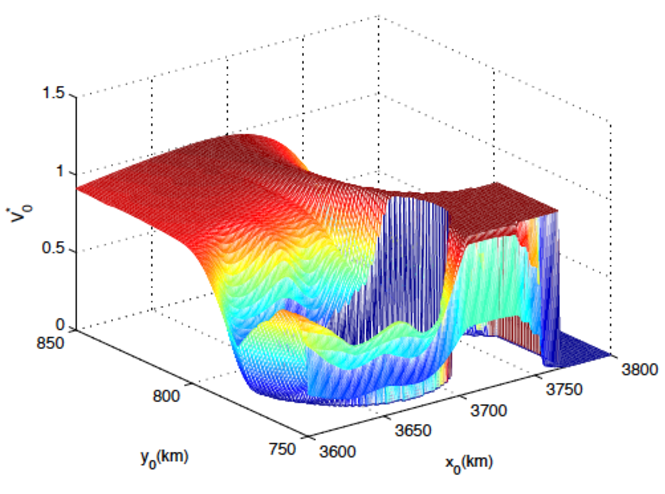
\includegraphics{img/Ch4ProbDecoupled}}                
                       \subfigure[Maximally safe trajectory]{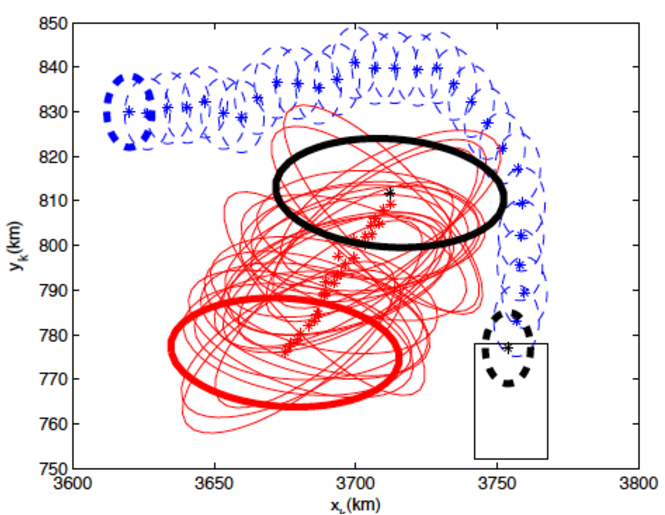
\includegraphics{img/Ch4PathDecoupled}}
                     \end{subfigmatrix}
                     \caption{Aircraft trajectory planning in stochastic environment}
                     \label{fig:prob_decoupled}
                   \end{center}
                 \end{figure}




               \subsubsection{Finite State Machines and Modal Models in Ptolemy II (Lee)}


               FSMs are actors whose behavior is described using a
               finite set of states and transitions between the
               states. The transitions between the states are enabled
               by guards, which are boolean-valued expressions that
               can reference inputs to the actor and parameters in
               scope. The transitions can produce outputs and can
               update the value of parameters in scope. Modal models
               extend FSMs by allowing states to have refinements,
               which are hierarchical Ptolemy II models. The
               refinements may themselves be FSMs, modal models, or
               any composite actor containing a director compatible
               with the domain in which the modal model is being
               used. On the basis of several examples, the memorandum
               describes the operational semantics, the practical
               usage, and the semantics of time in modal models.

               During this period, we released our update to the modal model system
               as part of Ptolemy II 8.0.1.  In addition we wrote a conference
               paper ``Modal Models in Ptolemy,''
               for the   Workshop on  Equation-Based Object-Oriented Modeling Languages and Tools,
               held in conjunction with MODELS
               \cite{LeeTripakis10_ModalModelsInPtolemyProceedings}
               \cite{LeeTripakis10_ModalModelsInPtolemyPresentation}, the
               abstract of which is reproduced below:
               \begin{quotation}
                 ``Ptolemy is an open-source and extensible modeling and simulation
                 framework. It offers heterogeneous modeling capabilities by allowing
                 different models of computation to be composed hierarchically in an
                 arbitrary fashion. This paper describes modal models, which allow to
                 hierarchically compose finite-state machines with other models of
                 computation, both untimed and timed. The semantics of modal models
                 in Ptolemy are defined in a modular manner.''
               \end{quotation}
               Model models were also covered in a
               general Ptolemy tutorial\cite{BrooksLeeTripakis10_ExploringModelsOfComputationWithPtolemyII}
               given at ESWeek 2010.



 

 \subsubsection{Verification of Hybrid Systems via Differential Invariants (Clarke, Platzer)}

Andr{\'e} Platzer has written a book about hybrid systems verification that will appear with Springer as "Logical Analysis of Hybrid Systems: Proving Theorems for Complex Dynamics." This book describes basic and advanced verification techniques for hybrid systems, including applications to air traffic control analysis. It will be a good introduction for graduate students working in the area.


\subsubsection{Embedded Convex Optimization (Boyd) }

This work concerns the use of convex optimization in high speed, real-time embedded systems, such as those found for signal processing, automatic control, estimation, resource allocation and decision making. While convex optimization is widely used on time scales of seconds or minutes, typically with a skilled engineer 'in the loop' supervising the optimization solver, it is less commonly seen for real-time applications.

A primary concern in real-time or embedded applications is the solver speed. We have ad-dressed this for a variety of applications, including using hand-coded solvers, including software for high-speed model predictive control (MPC).  Taking this work further, we have created an automatic code generator, CVXGEN, which takes a high-level description of a convex optimiza-tion problem and automatically generates compilable, library-free C code for a high speed solver.

This enables extensive (automatic) customization for the problem at hand, and makes solution much faster than existing methods. While with a hand-written solver, even small changes in problem specification necessitated painstaking redesign, even a complete change only requires the use of CVXGEN to automatically generate new code. This, combined with extremely fast solvers that carry out convex optimization on millisecond or even microsecond time scales, means that many new applications are possible, particularly for embedded systems.

A parallel branch of work investigates high-speed control algorithms for use in linear stochastic control. Here we evaluate a control-Lyapunov policy at each time step. For small problems the associated QP can be solved explicitly, but for larger problems on-line optimization is re-quired. This means the control-Lyapunov policy is often considered excessively computationally intensive for real-time or embedded systems. We have demonstrated several techniques for accelerating evaluation of control-Lyapunov policies, including the pre-computation of certain quantities, and the use of performance bounds that enable much faster approximate policies to be used instead. The performance bounds are computed offline using linear matrix inequalities and semidefinite programming.

Another related area of investigation has been algorithms for distributed optimization. Distributed optimization allows us to divide up computation of more complicated problems across multiple processing cores for faster computation. We have studied methods such as Alternating Directions Method of Multipliers, which provide a framework for decomposing convex optimization problems. Each subproblem can be solved completely in parallel, and the cores only need to communicate very simple messages during processing. With ever growing size and complexity of databases and information, using distributed optimization is increasingly becoming important to a wide range of problems in control, machine learning, portfolio optimization, network flow and scheduling. This will allow many of these problems (that have traditionally been considered slow) to be solved very fast and in real-time. 


